%%%%%%%%%%%%%%%%%%%%%%%%%%%%%%%%%%%%%%%%%%%%%%%%%%%%%%%
% Math 3250 Combinatorics, University of Connecticut
%%%%%%%%%%%%%%%%%%%%%%%%%%%%%%%%%%%%%%%%%%%%%%%%%%%%%%%

% Anything after a percent sign is a comment.

% Necessary first line. \documentclass defines the type of document and some options (for example, try changing the font size (10pt or 11pt or 12pt).
\documentclass[10pt, oneside]{amsart}
\usepackage{enumerate} % to be able to enumerate a list using non-numbers
\usepackage{tikz}
%for hypertext references
\usepackage[colorlinks = true,
            linkcolor = blue,
            urlcolor  = blue,
            citecolor = red,
            anchorcolor = green]{hyperref}


\usepackage[letterpaper]{geometry} % from 2016
\geometry{tmargin=0.8in,bmargin=0.1in,lmargin=1.30in,rmargin=1.30in}
\voffset -0.3in

% The part of the tex file between the \documentclass and \begin{document} line is called the preamble.  Things having to do with setting up the document are done in the preamble.  You will not need to mess with it for now, except to change your name and the title of your document. 
% After adding your name next to author, head down to where it says "Start here"

\title{Math3250 Portfolio Problems 3}
%\author{}
\begin{document}



\begin{center}
\textbf{Cover Sheet (Math3250 Combinatorics)}
\end{center}

Your Names: NAME

\vfill 

Assignment: Portfolio Problems 3

\vfill 

\bigskip
In this class, you are encouraged to discuss the problems with anyone. You are also allowed to use any resources as long as you cite them.

Please cite the individuals and documents that have helped you in completing this assignment. 
The individuals cited should include all classmates with whom you have collaborated (even if they only act as a sounding board by listening to you during class group work).
Documents cited should include class textbooks and all web content you have consulted.
\\


Individuals:

\vfill
\vfill

Documents:

\vfill
\vfill

\newpage


\maketitle

% --------------------------------------------------------
%                         Start here
% --------------------------------------------------------


\textbf{Overleaf Setup.}
To upload this template file, you can first download it to your local machine and then upload it (by clicking the upload button on the top left).
Alternatively, you can create a new blank file (click on the button shaped like paper on the top left), name it ``main.tex", then copy and paste the content of this template file to ``main.tex".

Please put your answer inside of the ``proof" environment provided under each problem. 

\bigskip

\tableofcontents





\section{Favorite theorems or write your own problems}

Complete one of the following subsections.

\subsection{Theorems from class}
\begin{enumerate}[i.]
	\item What were three favorite theorems from class?	
	
	\item 
	Pick a theorem from one of the topics covered. (You may pick a theorem which has or has not been covered in class.)
	Recreate its proof here.
	
\end{enumerate}

\begin{proof}[Answer]
	Enter your answers here.
\end{proof}


\subsection{Create your own problem}
Write a problem (of medium difficulty) related to one or more topics covered in class. Explain your solution in details.

\begin{proof}[Answer]
	Enter your answers here.
\end{proof}



\bigskip 


\section{Pigeon Hole Principle}

Complete one of the following two subsections.




\subsection{Wednesdays}


The month of April 2020 has five Wednesdays. For any given year, determine the possible number of months that contain five Wednesdays.


\begin{proof}
	Insert proof
\end{proof}



\subsection{Initials}
Eight hundred students are enrolled in Multivariable Calculus courses at UConn one semester. Prove that at least two students have the same first name-last name abbreviation (for example, Alex Brianna Chu would be abbreviated A.C). 


\begin{proof}
	Insert proof
\end{proof}

\textbf{Partial credit.}
If you have trouble with above, do any problem from 
\href{https://egunawan.github.io/combinatorics/hw/wk2problems.pdf}
{Week2} for partial credit.



~




\section{Polygon diagonals}
Let $n\geq 4$. Consider a convex $n$-gon that is drawn in such a way that no three diagonals intersect in one point. How many intersection points do the diagonals have? (For example, if you draw a pentagon, there are five diagonals and five crossings.) Prove this. 

\textbf{Partial credit.}
If you have trouble with above,   do any problem from 
\href{https://egunawan.github.io/combinatorics/hw/wk4problems.pdf}
{Week4} for partial credit.





~ 


\section{Identities with binomial coefficients}


 Do one of the following two subsections. 
You should review B\'ona Sec 4.1, especially Theorem 4.6 (counting ways to choose a committee and then a president).


\subsection{An identity}
Let $n \geq 2$ be an integer.
Show that 
\[
\sum_{j=1}^n j^2 {n \choose j} = n (n+1) 2^{n-2}.
\]
Give a combinatorial proof and also a proof using the Binomial Theorem (see Thm 4.6). 

\begin{proof}
Insert proof
\end{proof}


\subsection{Another identity}
Let $k$ and $n$ be positive integers such that $k < n$. 
Show that 
\[
\sum_{j=k}^n {j \choose k } {n \choose j} =  {n \choose k} 2^{n-k}.
\]

\begin{proof}
	Insert proof
\end{proof}

\subsection*{Partial credit}
If you have trouble with the above, do any problem from 
\href{https://egunawan.github.io/combinatorics/hw/wk5problems.pdf}
{Week 5} for partial credit.












\section{Perfect matchings}

A \emph{matching} of a graph $G$ is a set $M$ of edges of $G$ such that no two edges in $M$ shares a vertex.
A \emph{perfect matching} $M$ of a graph $G$ is a matching $M$ such that 
every vertex of the graph  $G$ is incident to exactly one edge of the matching. (For more info on matchings, you can see Section 1.7 of the HHM textbook, but it's not necessary.)

Let $G_n$ be a graph with vertices $a_1,\dots, a_n, b_1,\dots, b_n$ arranged in two rows so that the $a_i$ are at the bottom and $b_i$ are at the top. 
$G_n$ has $n + 2(n-1)$ edges:
there are $n$ vertical edges of the form $\{a_i,b_i\}$, there are $n-1$ edges of the form $\{a_i,a_{i+1}\}$, and there are $n-1$ edges of the form $\{b_i,b_{i+1}\}$.
See figure for $G_n$, $n=1,\dots, 5$.

For each $n\geq 1$, Let $f_n$ be the number of perfect matchings of $G_n$.
 The perfect matchings of $G_n$ for $n=1,\dots, 5$ are given in the picture.

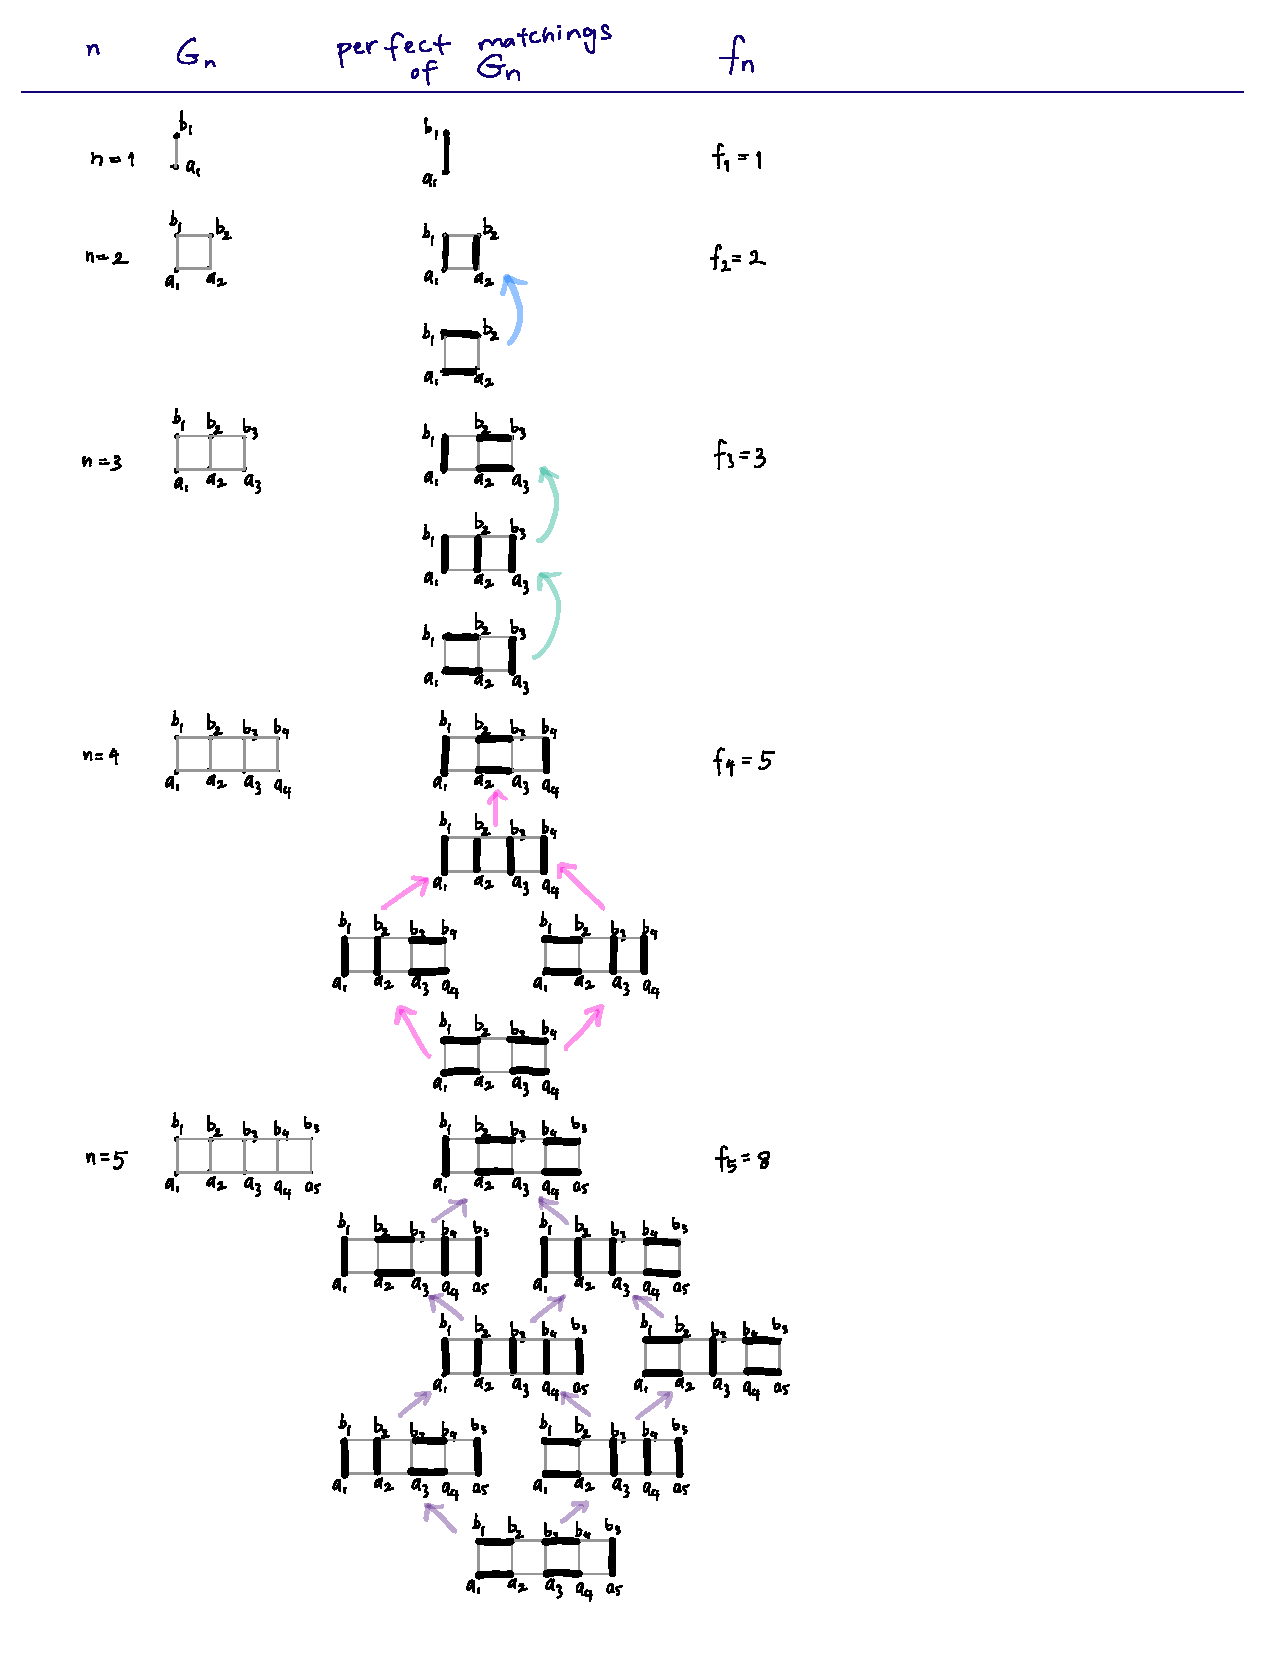
\includegraphics[height=8in]{portfolio3fig.pdf}



Complete at least two of the following three subsections.

\subsection{Recurrence relation}
\label{recurrence_relation}
Conjecture a recurrence relation for $f_n$. You've seen this many times.

~ 

(Optional)
Prove that your conjectured recurrence relation holds. Hint: Try using the same logic as in the proof of Theorem 4.3 (p. 74) of Bona. Given a perfect matching $M$ of $G_n$, break into two cases: either $M$ contains a perfect matching of $G_{n-1}$ or not.

\subsection{Generating function} 
Use Subsection \ref{recurrence_relation} to compute a closed form formula of a generating function (either ordinary or exponential) for $f_n$.


\subsection{Pattern observation}
Reference the figure. 
When is there an arrow from a perfect matching $M_1$ to a perfect matching $M_2$? What do you think is the rule to determine which perfect matching is drawn at the very bottom?  What perfect matching should be drawn at the very top?








\end{document}
